\documentclass [12pt] {article}

\usepackage{lscape,epsf,epsfig,natbib,amsfonts,amssymb,multirow,verbatim,tikz,float,amsmath,bbm,ulem,simplemargins,mathrsfs,amsthm,xspace}
\usetikzlibrary{shapes}

\newtheorem{prop}{Proposition}
\newtheorem{lemma}{Lemma}
\newtheorem{assu}{Assumption}
\newtheorem{remark}{Remark}
\newtheorem{defi}{Definition}
\newtheorem{theo}{Theorem}
\newtheorem{corr}{Corollary}
\newtheorem{exa}{Example}
\newtheorem{result}{Result}

\newcommand{\propr}[1]{{\bf Proof of Proposition \ref{#1}.}}
\newcommand{\respr}[1]{{\bf Proof of Result \ref{#1}.}}
\newcommand{\proo}{{\bf Proof }}

\bibliographystyle{econometrica}

\setleftmargin{0.75in}
\setrightmargin{0.75in}
\settopmargin{0.75in}
\setbottommargin{0.75in}
\DeclareMathAlphabet{\mathpzc}{OT1}{pzc}{m}{it}

%Shortcuts
\newcommand{\dwx}{\mathpzc{d}_w(x)}
\newcommand{\dex}{\mathpzc{d}_e(x)}
\newcommand{\dux}{\mathpzc{d}_u(x)}
\newcommand{\df}{\mathpzc{d}_f}
\newcommand{\dw}{\mathpzc{d}_w}
\newcommand{\dmxrho}{\mathpzc{d}_m(x,\rho)}
\newcommand{\dmxirho}{\mathpzc{d}_m(x_i,\rho)}
\newcommand{\dmxjrho}{\mathpzc{d}_m(x_j,\rho)}
\newcommand{\dm}{\mathpzc{d}_m}
\newcommand{\dmexrho}{\mathpzc{d}^*_m(x,\rho)}
\newcommand{\dvrho}{\mathpzc{d}_v(\rho)}
\newcommand{\dverho}{\mathpzc{d}^*_v(\rho)}
\newcommand{\B}{\mathcal{B}}
\newcommand{\dx}{\ \mathrm{d}x}
\newcommand{\dxi}{\ \mathrm{d}x_i}
\newcommand{\dxj}{\ \mathrm{d}x_j}
\newcommand{\indicator}[1]{\mathbbm{1}_{\left[ {#1} \right] }}

\newcommand{\Pbb}{\mathbb{P}}
\newcommand{\dmxy}{\mathpzc{d}_m}

\newcommand{\dmxtr}{\mathpzc{d}_m(\tilde{x},\rho)}
\newcommand{\dmxrt}{\mathpzc{d}_m(x,\tilde{\rho})}

\newcommand{\dvrt}{\mathpzc{d}_v(\tilde{\rho})}
\newcommand{\dr}{\mathrm{d}\rho}
\newcommand{\dtr}{\mathrm{d}\tilde{\rho}}
\newcommand{\dsp}{\mathpzc{d}_p}
\newcommand{\du}{\mathpzc{d}_u}
\newcommand{\dv}{\mathpzc{d}_v}
\newcommand{\mxtytoe}{\frac{\dh(\tilde{x},\tilde{y})}{E}}
\newcommand{\mxtytoedtxdty}{\frac{\dh(\tilde{x},\tilde{y})}{E} \ \mathrm{d}\tilde{x}\mathrm{d}\tilde{y}}
\newcommand{\ufytov}{\frac{\dv(\tilde{y})}{V}}
\newcommand{\ufyov}{\frac{\dv(y)}{V}}
\newcommand{\ufytovdty}{\frac{\dv(\tilde{y})}{V}\ \mathrm{d}\tilde{y}}
\newcommand{\uwxtoudtx}{\frac{\du(\tilde{x})}{U}\ \mathrm{d}\tilde{x}}
\newcommand{\uwxtou}{\frac{\du(\tilde{x})}{U}}
\newcommand{\uwxou}{\frac{\du(x)}{U}}
\newcommand{\Ce}{\mathbb{C}_e}
\newcommand{\Cu}{\mathbb{C}_u}
\newcommand{\Cp}{\mathbb{C}_p}
\newcommand{\Cv}{\mathbb{C}_v}
\newcommand{\Mu}{\mathbb{M}_u}
\newcommand{\Me}{\mathbb{M}_e}
\newcommand{\Mv}{\mathbb{M}_v}
\newcommand{\Mp}{\mathbb{M}_p}
\newcommand{\dtxdty}{\ \mathrm{d}\tilde{x}\mathrm{d}\tilde{y}}
\newcommand{\dtddr}{\ \mathrm{d}\tilde{\mathpzc{d}}_\rho(x)\mathrm{d}\tilde{\rho}}

\newcommand{\dtx}{\ \mathrm{d}\tilde{x}}
\newcommand{\dty}{\ \mathrm{d}\tilde{y}}
\newcommand{\drho}{\ \mathrm{d}\rho}
\newcommand{\dxdrho}{\ \mathrm{d}x\mathrm{d}\rho}
\newcommand{\tx}{\tilde{x}}
\newcommand{\ty}{\tilde{y}}
\newcommand{\by}{\bar{y}}
\newcommand{\dxdy}{\ \mathrm{d}x\mathrm{d}y}

\newcommand{\maxAux}{\max_{A(x)}\ \ }
\newcommand{\maxAvy}{\max_{A(y)}\ \ }
\newcommand{\Stxy}{S(\tilde{x},y)}
\newcommand{\Sxty}{S(x,\tilde{y})}
\newcommand{\iBvx}{\int\limits_{\Bvx}}
\newcommand{\iBpx}{\int\limits_{\Bpx}}
\newcommand{\iBuy}{\int\limits_{\Buy}}
\newcommand{\iBey}{\int\limits_{\Bey}}
\newcommand{\iBexy}{\int\limits_{\Bexy}}
\newcommand{\iBpxy}{\int\limits_{\Bpxy}}



\begin {document}
\title{\bf OTC\thanks{Thanks to ...}}
\author {
Garth Baughman \thanks{Department of Economics, University of Pennsylvania, 160 McNeil Building, 3718 Locust Walk, Philadelphia, PA, 19104-6297 USA. E-mail: garthb@sas.upenn.edu.}\\
Tzuo Hann Law \thanks{Department of Economics, University of Pennsylvania, 160 McNeil Building, 3718 Locust Walk, Philadelphia, PA, 19104-6297 USA. E-mail: tzuolaw@sas.upenn.edu.}
\\University of Pennsylvania \vspace{0.5in} \\ \vspace{0.5in} PRELIMINARY AND INCOMPLETE}
\date{\today}
\maketitle \vspace{-0.7cm}
\thispagestyle{empty}
\begin{abstract}
Search in OTC markets for exotic assets.
\end{abstract}
\newpage

%%%%%%%%%%%%%%%%%%%%%%%%%%%%%%%%%%%%%%%%%%%%%%%%%%%%%%%%%%%%%%%%%%%%%%%%%%%%%%%%%%%%%
%%%%%%%%%%%%%%%%%%%%%%%%%%%%%%%%%%%%%%%%%%%%%%%%%%%%%%%%%%%%%%%%%%%%%%%%%%%%%%%%%%%%%
%%%%%%%%%%%%%%%%%%%%%%%%%%%%%%%%%%%%%%%%%%%%%%%%%%%%%%%%%%%%%%%%%%%%%%%%%%%%%%%%%%%%%
%%%%%%%%%%%%%%%%%%%%%%%%%%%%%%%%%%%%%%%%%%%%%%%%%%%%%%%%%%%%%%%%%%%%%%%%%%%%%%%%%%%%%

\section{Introduction}\label{section:introduction}
PLACEHOLDER

%%%%%%%%%%%%%%%%%%%%%%%%%%%%%%%%%%%%%%%%%%%%%%%%%%%%%%%%%%%%%%%%%%%%%%%%%%%%%%%%%%%%%
%%%%%%%%%%%%%%%%%%%%%%%%%%%%%%%%%%%%%%%%%%%%%%%%%%%%%%%%%%%%%%%%%%%%%%%%%%%%%%%%%%%%%
%%%%%%%%%%%%%%%%%%%%%%%%%%%%%%%%%%%%%%%%%%%%%%%%%%%%%%%%%%%%%%%%%%%%%%%%%%%%%%%%%%%%%
%%%%%%%%%%%%%%%%%%%%%%%%%%%%%%%%%%%%%%%%%%%%%%%%%%%%%%%%%%%%%%%%%%%%%%%%%%%%%%%%%%%%%
\section{Baseline model}\label{section:model}
\subsection{Banks}
There are a finite number $ N $ of infinitely lived banks who discount the future at rate $ \beta $. At the beginning of each period, bank $ i $ is described by two scalars, working capital and risky assets, which we denote by $ (D_{i,t},B_{i,t}) $. Banks partition working capital into a liquid form, ``money'', $ M_{i,t} $ which bear no returns, or, an illiquid form, ``loans'', $ L_{i,t} $ which bear constant interest $ 1 + r $. There are sub-periods in each $ t $. We assume that all information is public. As variables change from period to period, we use $ t' $ to denote the first instance where a variable changes within period, $ t'' $ to denote the same variable after the second change, and so on.
\begin{enumerate}
\item \textbf{Wealth shock.} All banks experience IID shock $ w_{i,t} $ to $ D_{i,t} $. 
\[ D_{i,t'} = D_{i,t} + w_{i,t} \]
\item \textbf{Frictional markets.} One randomly selected bank is allowed to post one TIOLI fixed-for-floating offer. Denote the change in a bank's working capital position from trade by $ \Delta^D_{i,t} $ and the change in the risky asset position by $ \Delta^B_{i,t} $.
\[ D_{i,t''} = D_{i,t'} +  \Delta^D_{i,t} \]
\[ B_{i,t'}  = B_{i,t} +  \Delta^B_{i,t} \]
\item \textbf{Reallocation.} Banks decide on $ M_{i,t} $ and $ L_{i,t} $ such that 
\[ M_{i,t} + L_{i,t} = D_{i,t''}. \]
\item \textbf{Risky returns.} With probability $ \lambda $ which is independent across firms, risky assets post returns $ r^B_{i,t} $ which may be negative. If risky returns are realized, a banks change in its money holdings is 
\[ \Delta^M_{i,t} = M_{i,t} + r^B_{i,t}B_{i,t'}. \] 
\[ M_{i,t'} = \Delta^M_{i,t} + M_{i,t} \] 
If $ M_{i,t'} < 0 $ a kitten dies.
\item \textbf{Risk-free return.} \[ L_{i,t'} = (1+r)L_{i,t} \]
\item \textbf{Competitive market.} All banks participate in a competitive fixed-for-floating market.
\[ q_tB_{i,t+1} + D_{i,t+1} = q_{t}B_{i,t'} + L_{i,t'} + M_{i,t'} \]
\end{enumerate}
In graphical form, the events in 1 periods follow
\begin{figure}[H]
\begin{center}
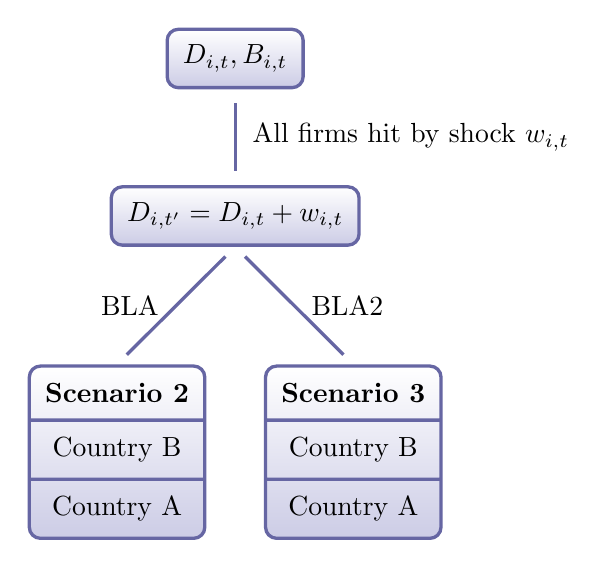
\begin{tikzpicture}[
    grow=down,
    level 1/.style={sibling distance=3cm, level distance=2cm},
    level 2/.style={sibling distance=3cm, level distance=3cm},
    level 3/.style={sibling distance=3cm, level distance=2cm},
    edge from parent/.style={very thick,draw=blue!40!black!60,shorten >=5pt, shorten <=5pt},
    edge from parent path={(\tikzparentnode.south) -- (\tikzchildnode.north)},
    kant/.style={text centered},
    every node/.style={text ragged, inner sep=2mm},
    punkt/.style={rectangle,rounded corners,shade,top color=white,bottom color=blue!50!black!20,draw=blue!40!black!60,very thick}
    ]
\node[punkt] {$ D_{i,t},B_{i,t}$}
    %Upper part, lv1
    child {
        node[punkt] {$ D_{i,t'} = D_{i,t} + w_{i,t} $}
        %child 1
        child {
            node [punkt,rectangle split, rectangle split,
            rectangle split parts=3] {
                \textbf{Scenario  2}
                \nodepart{second}
                $\text{Country B}$
                \nodepart{third}
                $\text{Country A}$
            }
            edge from parent
                node[left, kant,  pos=.5] {BLA}
        }
        %child 2
        child {
            node [punkt, rectangle split, rectangle split parts=3]{
                \textbf{Scenario 3}
                \nodepart{second}
                $\text{Country B}$
                \nodepart{third}
                $\text{Country A}$
            }
            edge from parent
                node[kant, right] {BLA2}
                }
            edge from parent{
                node[kant,right,pos = 0.5] {All firms hit by shock $ w_{i,t} $}
                }
 };
\end{tikzpicture}
\end{center}
\end{figure}

\section{Empirics}
PLACEHOLDER

\section{Conclusion}
PLACEHOLDER

\section{Extensions}
PLACEHOLDER



\bibliography{C:/Users/tzuohann/Desktop/Dropbox/Research/PaperCollection/Bibliography}
%\bibliography{/home/tzuohann/Dropbox/Research/PaperCollection/Bibliography}
\end{document} 
}
